 \subsection{Cremmer-Gervais $i \mapsto i-1$}
The initial quiver for $\gc_h^{\dagger}(\bg,\GL_4)$ is illustrated in Figure~\ref{f:n=4_CG_i-i-1}.

\begin{figure}[htb]
\begin{center}
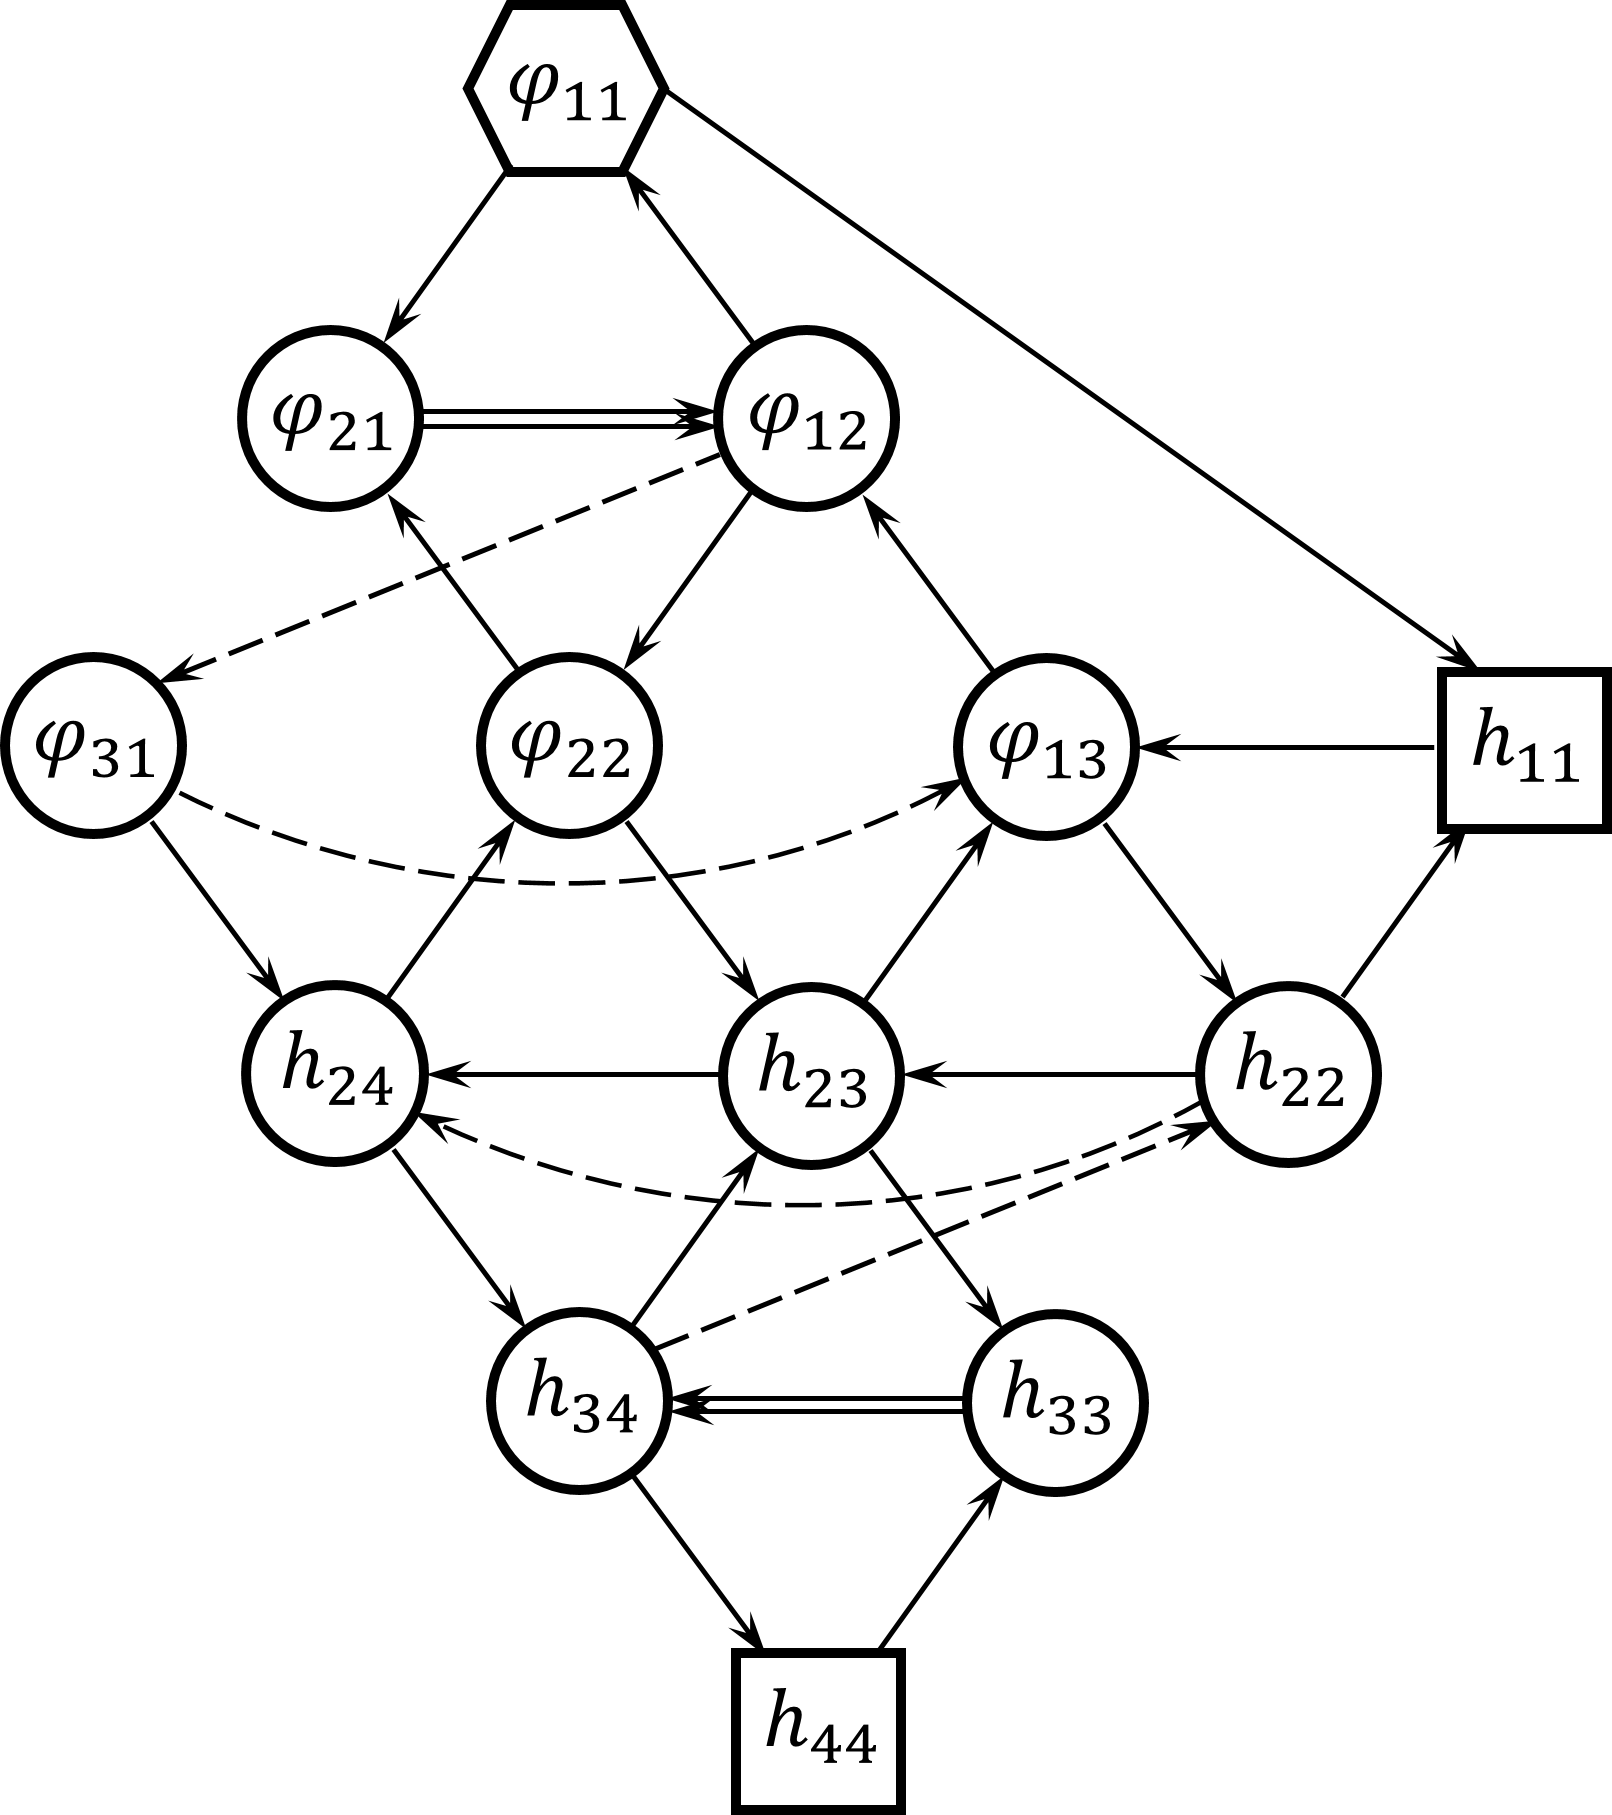
\includegraphics[scale=0.65]{h_convention/h_n=4_CG_i-i-1.png}
\end{center}
\caption{The initial quiver for $\gc^{\dagger}_g(\bg,\GL_4)$ for $\Gamma_1 = \{2,3\}$, $\Gamma_2 = \{1,2\}$, $\gamma:i \mapsto i-1$.}
\label{f:n=4_CG_i-i-1}
\end{figure}
 
 \paragraph{The initial variables.} In the initial extended cluster, all cluster and frozen variables are given as in $\gc_h^{\dagger}(\bg_{\std},\GL_4)$ except for the variables $h_{34}$, $h_{33}$, $h_{44}$. These are given by:
\begin{align}
    &h_{34}(U) = -u_{34}\det U^{[2,4]}_{[2,4]} - u_{24} \det U^{\{1\}\cup[3,4]}_{[2,4]};\\
    &h_{33}(U) = \det U^{[3,4]}_{[3,4]} \det U^{[2,4]}_{[2,4]} + \det U^{[3,4]}_{\{2,4\}} \det U^{\{1\}\cup[3,4]}_{[2,4]} + \det U^{[3,4]}_{[2,3]}\det U^{[1,2]\cup\{4\}}_{[2,4]};
\end{align}
\begin{equation}
    \begin{split}
     h_{44}(U) = &u_{44}\left(\det U^{[3,4]}_{[3,4]} \det U^{[2,4]}_{[2,4]} + \det U^{[3,4]}_{\{2,4\}} \det U^{\{1\}\cup[3,4]}_{[2,4]} + \det U^{[3,4]}_{[2,3]}\det U^{[1,2]\cup\{4\}}_{[2,4]}\right) + \\ + &u_{34}\left(\det U^{\{2,4\}}_{[3,4]} \det U^{[2,4]}_{[2,4]} + \det U^{\{2,4\}}_{\{2,4\}} \det U^{\{1\}\cup[3,4]}_{[2,4]} + \det U^{\{2,4\}}_{[2,3]}\det U^{[1,2]\cup\{4\}}_{[2,4]}\right) + \\ + &u_{24}\left(\det U^{\{1,4\}}_{[3,4]} \det U^{[2,4]}_{[2,4]} + \det U^{\{1,4\}}_{\{2,4\}} \det U^{\{1\}\cup[3,4]}_{[2,4]} + \det U^{\{1,4\}}_{[2,3]}\det U^{[1,2]\cup\{4\}}_{[2,4]}\right).
    \end{split}
\end{equation}

\paragraph{Birational quasi-isomorphisms.} TBD